\chapter{OpenID Based Solution}
\section{Introduction}
In this chapter we will provide a solution using OpenID based IMS. We will give more details about how this system can be implemented, and how will it behave for the end users.
\section{OpenID IMS}
We can replace IMS with OpenID based IMS in our pseudonymous system. This system will take user credentials and then send Pseudonym, Account ID and Policy to the bank. This IMS can be controlled by a separate identity inside the bank or by a 3rd party.
\begin{figure}[h]
	\centering
	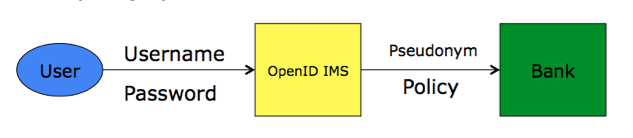
\includegraphics[width=\textwidth]{figures/OpenID}
	\caption{Pseudonym System with OpenID IMS}
	\label{fig:OpenID}
\end{figure}
\section{System Setup}
The system can be setup in 2 ways:
\begin{itemize}
	\item IMS controlled by a separate department at bank.\\
	In this case the bank separate the authentication and service part in 2 different departments internally. Authentication is controlled by IMS which holds the sensitive user data but the service department doesn't need to have access to that data to provide service to the user.
	\item IMS controlled by a third party\\
	In this case the bank operates the service part while the authentication part is operated by a trusted third party.
\end{itemize}
In both cases, bank and IMS have to collaborate and bank have to trust the IMS system that pseudonym and policy sent by the IMS system is correct.
\subsection{Changes on the Bank Side}
In order to provide services to a pseudonym bank needs to have a temporary policy database at its end. So that when bank gets the pseudonym and policy from the IMS system, it can store that policy with the pseudonym and provide the services according to the policy.
\subsection{Information Stored at IMS}
IMS need following user information to be stored
\begin{itemize}
	\item User ID
	\item Account ID
	\item Policy
\end{itemize}
Account ID and policy can be stored in encrypted form, which can then only be opened by the bank. OpenID IMS also need to store a mapping database from User ID to Pseudonym for escrow purposes.
\subsection{Changes needed on the User Side}
On user side no changes are needed. User access the system like before. User doesn't need to install any special software or hardware on his side to access the bank services. 
\section{User Creation}
Following are the steps for creation of a new user account in OpenID based system
\begin{itemize}
	\item User goes to bank to open a new account.
	\item User provides his details.
	\item Bank creates user policy and send this information to the IMS system along with other user information.
	\item IMS system verifies the user information and provides user with credentials to access his account.
	\item User then can login to his account using the credentials.
	\item In case of corporate users, if user is the administrator then he can add more users using a web interface at the IMS system directly and decide account policies for those users.
\end{itemize}
\section{User Authentication}
Authentication steps are as following in OpenID based system
\begin{itemize}
	\item User goes to login page
	\item User provides his username and password
	\item This is sent to OpenID IMS which verifies the user and creates a pseudonym for the given user ID
	\item This user ID to pseudonym mapping is stored in the database for escrow purposes
	\item IMS gets the policy for the given user ID from the policy database
	\item IMS then sends the pseudonym, Account ID and Policy to the bank 
	\item Bank gets this information and create a temporary policy for the given pseudonym
	\item User can then access services from the bank using the pseudonym
	\item All user transactions are logged with the pseudonym
\end{itemize}
\section{ID Escrow}
Following are the steps for ID escrow in OpenID based system
\begin{itemize}
	\item Authorities come to the bank for transaction data.
	\item After verifying, bank gives the transaction data to the authorities.
	\item Authorities then go to the IMS based system for the mapping data.
	\item After verifying, IMS gives the mapping data to the authorities.
	\item Authorities then get the real identity of the user from mapping and transaction data.
\end{itemize}
\section{Analysis}
With the use of OpenID IMS we add a pseudonymous layer in the system. This provides us the necessary privacy. But in order to do so OpenID provider needs access to a lot of data. Some of the example data is:
\begin{itemize}
	\item UserID
	\item Account ID 
	\item Policies	
\end{itemize}
In addition to that, the provider needs to store the mapping database from UserID to Pseudonym. Bank really has to trust the provider with storage of all this sensitive data. In some cases bank might not want the provider to store such data by themselves.
\\
\\In case there is a discrepancy, the authorities need to go both to the bank to get the transaction data as well as the provider for the mapping data.
\section {OpenID implementation in the Real World}
Now we will try to fit this implementation in our system, which includes Nykredit as the Bank, Signicat as the 3rd party, DTU as corporate customer and other government institutions as authorities.
\subsection{Addition of the New User}
Addition of the new user can happen as following:
\begin{enumerate}
	\item DTU registers the new user with the Nykredit giving them the user details and policies that should apply to the particular user regarding the account. 
	\begin{enumerate}
		\item Nykredit registers this new user with his User ID with the IMS system. Nykredit also add policy for the user in the IMS system.
	\end{enumerate}
	\item Nykredit issue a user credentials for the given user to DTU.
	\item DTU then use this policy credentials to register the new user with Signicat. 
	\begin{enumerate}
		\item Signicat inquire about the user data with the authorities
		\item Authorities verify the user data to Signicat
	\end{enumerate}
	\item After that Signicat issue final OpenID credentials for the IMS system.  This credential is then used to login to the IMS system by the new user.
\end{enumerate}
\begin{figure}[h]
	\centering
	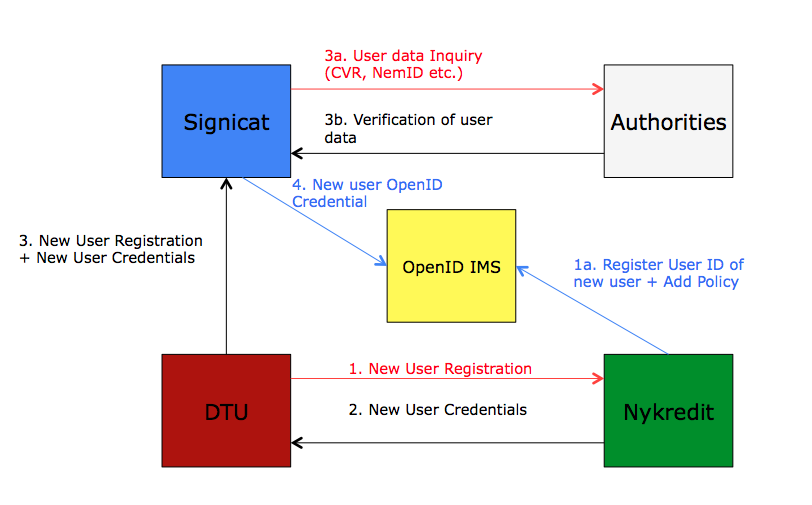
\includegraphics[width=\textwidth]{figures/OpenID-Real}
	\caption{OpenID Registration for a new user}
	\label{fig:OpenID-Real}
\end{figure}

\FloatBarrier
\subsection{Addition of a New Customer}
Addition of the new customer is almost same as addition of new user:
\begin{enumerate}
	\item An administrator goes to Nykredit to open a bank account on behalf of DTU 
	\begin{enumerate}
		\item Nykredit registers DTU as new customer in their internal system.
		\item Nykredit register the DTU administrator with his User ID with the IMS system
	\end{enumerate}
	\item Nykredit issue user credentials for the  DTU administrator to himself.
	\item Administrator then use these credentials to register himslef as owner of the new DTU account with Signicat. 
	\begin{enumerate}
		\item Signicat inquire about the data given in the credential with the authorities
		\item Authorities verify the dta to Signicat
	\end{enumerate}
	\item After that Signicat issue final OpenID credential for the IMS system. This credential is then used to login to the IMS system by the administrator.
\end{enumerate}
\subsection{Technical Requirements}
In this system DTU as a client doesn't need to change anything on their side to be a customer at Nykredit. All the system for DTU is web based where they can just add/remove users and also DTU users login to the system using the browser.
\\
\\Nykredit have to implement OpenID relying party service on their side. In this case they have to store sensitive data with the 3rd party. The account details and policies are stored at IMS.
\\
\\Signicat have to implement OpenID identity provider service on their side.
\\\\
IMS have to implement  OpenID identity provider service on their side.
\section{Summary}
This chapter described the IMS system setup using the OpenID system. We described how the system will be setup and how it will affect all the parties involved. Finally we discussed how OpenID IMS will be implemented in the real world scenario.

